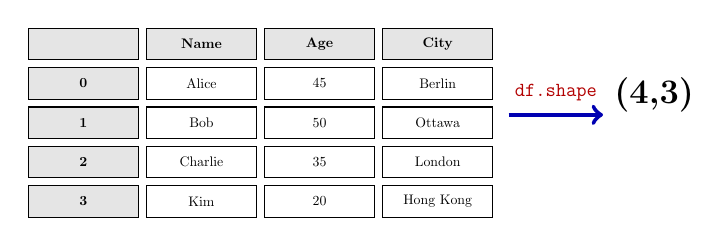
\begin{tikzpicture}[scale=0.5, transform shape,
    cell/.style={
        draw,
        minimum width=2.8cm,
        minimum height=0.8cm,
        align=center
    },
    header/.style={
        cell,
        fill=gray!20,
        font=\bfseries
    }
]

%%%%%%%%%%%%%%%%%%%%%%%%
% DataFrame original
%%%%%%%%%%%%%%%%%%%%%%%%

% --- Headers ---
\node[header] at (0,0) {};
\node[header] at (3,0) {Name};
\node[header] at (6,0) {Age};
\node[header] at (9,0) {City};

% --- Row 0 ---
\node[header] at (0,-1) {0};
\node[cell] at (3,-1) {Alice};
\node[cell] at (6,-1) {45};
\node[cell] at (9,-1) {Berlin};

% --- Row 1 ---
\node[header] at (0,-2) {1};
\node[cell] at (3,-2) {Bob};
\node[cell] at (6,-2) {50};
\node[cell] at (9,-2) {Ottawa};

% --- Row 2 ---
\node[header] at (0,-3) {2};
\node[cell] at (3,-3) {Charlie};
\node[cell] at (6,-3) {35};
\node[cell] at (9,-3) {London};

% --- Row 3 ---
\node[header] at (0,-4) {3};
\node[cell] at (3,-4) {Kim};
\node[cell] at (6,-4) {20};
\node[cell] at (9,-4) {Hong Kong};

%%%%%%%%%%%%%%%%%%%%%%%%
% Flecha df.iloc[0]
%%%%%%%%%%%%%%%%%%%%%%%%

\draw[->, ultra thick, blue!70!black]
    (10.8,-1.8)
    to[out=0,in=180]
    node[midway, above=6pt,
          font=\ttfamily\Large,
          text=red!70!black]
    {df.shape}
    (13.2,-1.8);

%%%%%%%%%%%%%%%%%%%%%%%%
% Resultado df.iloc[0] como Series
%%%%%%%%%%%%%%%%%%%%%%%%

% Título
\node[font=\bfseries\Huge] at (14.5,-1.3) { (4,3) };

%\node[font=\ttfamily\small] at (19.5,-4.2) {Name: 0};

\end{tikzpicture}
